%%=============================================================================
%% De zoektocht naar een gepast doel voor de spraakassistent
%%=============================================================================

\chapter{Een gepast doel voor de spraakassistent}
\label{ch:zoektocht}

\section{Ondersteuning van de begeleider in de jeugdzorg}
\label{ondersteuning van de begeleider in de jeugdzorg}
De aanleiding van dit onderzoek was een onderzoek van \textcite{Buysse} over faciliterende IT bij individuele begeleidingsgesprekken in de jeugdzorg. Uit het onderzoek ontstond er twijfel over het gebruik van een spraakassistent als ondersteuning bij het individuele begeleidingsgesprek tussen de persoonlijke begeleider en het kind. Door de twijfel werd er dan ook beslist om niet verder te gaan met spraaktechnologie, maar met andere digitale tools.

Om er toch zeker van te zijn dat er geen mogelijkheden waren, ontstond deze bachelorproef. Echter, na een eerste gesprek met Iris Storme, docent orthopedagogie binnen Hogeschool Gent en tevens mede-researcher van \textcite{Buysse} werden voor mij de beweegredenen voor het afkeuren van spraaktechnologie binnen hun onderzoek snel duidelijk. 

Als je denkt aan mensen met een visuele of fysieke beperking komen er snel mogelijkheden naar boven. Denk maar aan het controleren van apparaten met een eenvoudig stemcommando. Deze personen kunnen technologie als een mogelijke oplossing zien, waardoor zij, en de begeleiders, dit gemakkelijker kunnen omarmen.
Daartegenover staat de bijzondere jeugdzorg, waar de spraakassistent eerder ondersteuning zou bieden in de emotionele problematiek en de jongeren net hun façade nodig hebben om overeind te blijven. Deze doelgroep stelt zich niet zo graag kwetsbaar op en ervaart het praten over gevoelens eerder als een drempel. De bijzondere jeugdzorg lijkt op het eerste zicht een minder relevante doelgroep.

Dit werd allemaal vastgesteld door het intuïtieve gevoel van de ondervraagde. Dit was voor mij persoonlijk voldoende om te gaan nadenken over een nieuwe doelgroep.

\section{Ondersteuning van personen met het syndroom van Down}
\label{ondersteuning van personen met het syndroom van Down}
Ik wijzigde mijn doelgroep naar personen die geboren zijn met trisomie 21, ook wel het syndroom van Down genoemd. Uit een eerste opzoeking stelde ik de volgende mogelijkheden.

Personen met het Downsyndroom worden geboren met een verstandelijke beperking. Er kan gekeken worden naar welke noden uit die verstandelijke beperking vloeien, bijvoorbeeld moeite met rekenen, en hoe een spraakassistent hier ondersteuning kan bieden. Dit kan ook veel verder gaan als in vb. het helpen met zelfstandig wonen.

Daarnaast zijn er ook mogelijke bijkomende aandoeningen zoals een minder goed geheugen, coeliakie, slaapapneu, oogafwijkingen of een gedragsstoornis. Hier kan spraakassistentie mogelijks ook ondersteuning in bieden. Ik denk aan bijvoorbeeld interactieve activiteiten voor het stimuleren van de motoriek, het geheugen of het spraakvermogen, helpen herinneren aan belangrijke taken, helpen herinneren aan wat ze wel of niet mogen eten, stimuleren van een vast slaappatroon, enzovoort. \autocite{Volksgezondheidenzorg2019}

Dit waren nog maar losse ideeën die ontstonden uit een eerste verkenning over personen met het gendefect. Het werd duidelijk dat hier zeker mogelijkheden waren, dus was de volgende stap om hierin te gaan verdiepen door interviews af te nemen van mensen die een persoonlijke ervaring hebben met deze doelgroep.

Echter, mijn eerste aanvraag voor een interview aan iemand wiens dochter geboren is met trisomie 21 stootte direct op weerstand. Het antwoord dat ik kreeg, ging over het gevaar van veralgemenen. Het is een complexe materie omdat het gaat over een combinatie van samenkomende symptomen en kenmerken. De effecten van het gendefect kunnen in verschillende gradaties voorkomen, waardoor elke persoon die het gendefect bezit uniek moet bekeken worden.

Daarnaast kwam ik te weten dat ik niet zomaar zonder ervaring met een bijzondere doelgroep kan werken. Het wordt door veel deskundigen in de sector afgeraden en meestal is er ook toestemming voor nodig.
Het werd me duidelijk dat werken met een doelgroep die bijzondere hulp nodig heeft niet aangewezen is. Als dit echt de bedoeling is, dan is het raadzaam om samen te werken met een deskundige in de sector.

\section{Verlenen van eerste hulp bij ongevallen}
Op 2 april 2019 kwam het Rode Kruis met de lancering van een mobiele applicatie voor het geven van eerste hulp bij ongevallen. Dit gaf me de aanleiding om mijn onderzoek hier naar te richten.

\begin{figure}[h]
    \centering
    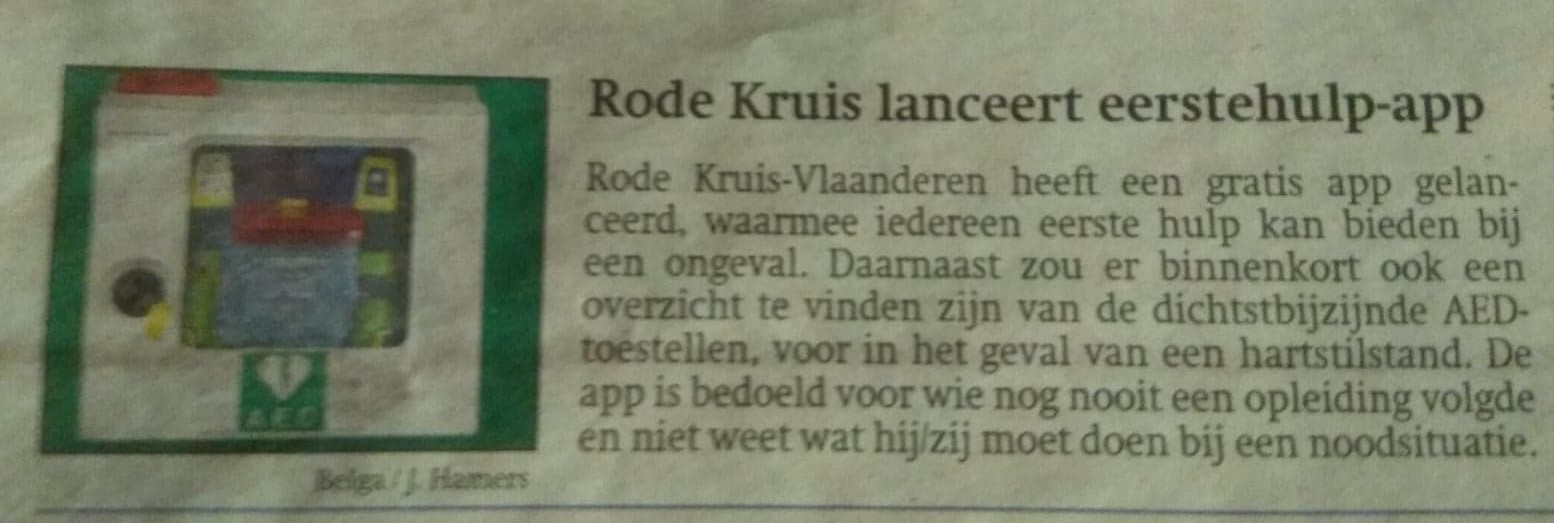
\includegraphics[width=0.8\linewidth]{img/artikelRodeKruisApp}
    \caption{Het artikel over de lancering. \autocite{Hamers2019}}
    \label{fig:artikel-ehboapp}
\end{figure}

Na het lezen van het artikel begon ik na te denken over de voordelen van een soortgelijke applicatie voor een spraakassistent. Als er tijdens de situatie een smart speaker in de buurt is, bijvoorbeeld thuis of op kantoor, dan hoeft de hulpverlener alleen maar de nodige instructies te vragen aan de assistent van de smart speaker. Als dit niet het geval is kan de applicatie mogelijks geopend worden via een spraakassistent op de smartphone. Omdat het belangrijk is om de handen steeds vrij te hebben om de nodige hulp toe te dienen, is de instructies vragen met de stem een groot voordeel.

Bij het gebruik van de mobiele applicatie had ik persoonlijk mijn twijfels. In een noodsituatie kan de hulpverlener in paniek zijn en dan is het niet aangewezen om nog de smartphone te moeten zoeken en de applicatie te openen. In de lijst van ongevallen moet dan nog de juiste situatie geselecteerd worden voordat de instructies leesbaar of hoorbaar zijn. Smartphones staan meestal ingesteld dat ze na een verlopen tijd in slaapstand gaan. Als iemand bezig is met hulp verlenen en de volgende stap wilt weten, kan het voorvallen dat de smartphone zich in slaapstand bevindt.

De applicatie is niet gericht op een bijzondere doelgroep, maar is bruikbaar voor iedereen bij een ongeval. Dit zorgt dat ik niet op dezelfde muur zal stoten van bij mijn vorige opties.